\documentclass{article}

% if you need to pass options to natbib, use, e.g.:
%     \PassOptionsToPackage{numbers, compress}{natbib}
% before loading neurips_2020

% ready for submission
%\usepackage{neurips_2020}

% to compile a preprint version, e.g., for submission to arXiv, add add the
% [preprint] option:
%     \usepackage[preprint]{neurips_2020}

% to compile a camera-ready version, add the [final] option, e.g.:
%     \usepackage[final]{neurips_2020}

% to avoid loading the natbib package, add option nonatbib:
\usepackage{natbib}
\usepackage[final]{neurips_2020}

\usepackage[utf8]{inputenc} % allow utf-8 input
\usepackage[T1]{fontenc}    % use 8-bit T1 fonts
\usepackage{hyperref}       % hyperlinks
\usepackage{url}            % simple URL typesetting
\usepackage{booktabs}       % professional-quality tables
\usepackage{amsfonts}       % blackboard math symbols
\usepackage{amsmath}
\usepackage{nicefrac}       % compact symbols for 1/2, etc.
\usepackage{microtype}      % microtypography
\usepackage{hyperref}
\usepackage{soul}
\usepackage{etoolbox}
\usepackage{graphicx}
\usepackage{multirow}
\usepackage{tabu}
\usepackage[dvipsnames, table,xcdraw]{xcolor}
\usepackage{etoolbox,refcount}
\usepackage{multicol}
\usepackage[font={small,it}]{caption}
\usepackage{subcaption}
\usepackage[title]{appendix}

\newcounter{countitems}
\newcounter{nextitemizecount}
\newcommand{\setupcountitems}{%
  \stepcounter{nextitemizecount}%
  \setcounter{countitems}{0}%
  \preto\item{\stepcounter{countitems}}%
}
\makeatletter
\newcommand{\computecountitems}{%
  \edef\@currentlabel{\number\c@countitems}%
  \label{countitems@\number\numexpr\value{nextitemizecount}-1\relax}%
}
\newcommand{\nextitemizecount}{%
  \getrefnumber{countitems@\number\c@nextitemizecount}%
}
\newcommand{\previtemizecount}{%
  \getrefnumber{countitems@\number\numexpr\value{nextitemizecount}-1\relax}%
}
\graphicspath{ {./images/} }
\makeatother    
\newenvironment{AutoMultiColItemize}{%
\ifnumcomp{\nextitemizecount}{>}{3}{\begin{multicols}{2}}{}%
\setupcountitems\begin{itemize}}%
{\end{itemize}%
\unskip\computecountitems\ifnumcomp{\previtemizecount}{>}{3}{\end{multicols}}{}}

\title{Analysing Traffic through Emulation}

% The \author macro works with any number of authors. There are two commands
% used to separate the names and addresses of multiple authors: \And and \AND.
%
% Using \And between authors leaves it to LaTeX to determine where to break the
% lines. Using \AND forces a line break at that point. So, if LaTeX puts 3 of 4
% authors names on the first line, and the last on the second line, try using
% \AND instead of \And before the third author name.
\newbool{showComments}
\booltrue{showComments}
% \boolfalse{showComments}

\ifbool{showComments}{%
\newcommand{\harry}[1]{\sethlcolor{green}\hl{[Harry: #1]}}
\newcommand{\matteo}[1]{\sethlcolor{red}\hl{[Matteo: #1]}}
\newcommand{\nicholas}[1]{\sethlcolor{cyan}\hl{[Nicholas: #1]}}
\newcommand{\new}[1]{\textcolor{blue}{#1}}
}{
\newcommand{\harry}[1]{}
\newcommand{\del}[1]{}
\newcommand{\new}[1]{}
}
\author{%
  Matteo Bettini \\
  mb2389 \\
  Sidney Sussex College\\
  % examples of more authors
  \And
  Nicholas Kastanos \\
  nk569 \\
  Queens' College \\
  \And
  Harry Songhurst \\
  hs778 \\
  St Edmund's College \\
}

\begin{document}

\maketitle

\begin{abstract}
    Urban planning and traffic management is a growing issue. In order to plan for rapidly urbanising populations, government agencies and local councils need to consider multiple factors, including traffic flow and air quality. Traditional large-scale traffic simulations are resource and time-intensive, especially when simulating microscopic details. Gaussian Processes fitted to simulation data can be used to model the input-output relationships of the system without the complexity of the simulator. In this project, the SUMO traffic simulator is used to create traffic flow and carbon dioxide emulation models for city-centre-like grid road networks through Experimental Design. Once the models have been developed, Bayesian Optimisation techniques are used to locate the optimal configuration of each model to reduce time lost by vehicles, and CO$_2$ emissions. The sensitivity of the models to each input parameter is then analysed. It is shown that the optimal operating point has low maximum vehicle speeds and accelerations, with long road lengths. An important trade-off exists between the two outputs with respect to the city size. The most significant input is the maximum vehicle speed.
\end{abstract}


% \harry{Targeting about 4000 words}

\section{Introduction and Motivation}
Since 1950, the proportion of the world's population living in urban areas has increased from 30\% to approximately 55\%. This trend is projected to continue, with an expected 60\% of the world's population living in cities by 2030 \cite{bravo2018sustainable}. With denser concentrations of people comes denser concentrations of cars and other vehicles, and thus the need for better urban planning, traffic management, and, where necessary, laws restricting the usage of motor-vehicles all together.

Government agencies and local councils often confront these challenges with multiple objectives in mind; improving air quality, improving traffic flow, and improving road safety, to name a few. To understand the effect that various confounding factors have on these measures, urban planners have many tools at their disposal such as air quality surveying, traffic monitoring, and perhaps most importantly, running vast and detailed simulations of cars moving through virtual reconstructions of the area they wish to understand.

For simulations to be representative and reliable, they must look at large areas and simulate the movement of tens of thousands of vehicles. This can be \textit{extremely} computationally expensive, especially if we care about collecting highly granular data at every step of the simulation. 

% This project explores how emulation can be employed to build models of traffic simulators. Our emulators provide a solution that is much faster to run, while also allowing us to analyse the relative importance of input factors affecting the simulation as well as optimise the road network and the vehicles to tackle specific objectives (e.g., reduction of traffic congestion, reduction in CO2 emissions). Taken to production quality, such an emulator could inform time-sensitive decisions that urban planners could take into account when designing the cities of the future.
This project explores how emulation can be employed to build models of traffic simulators. Specifically, we consider the problems of predicting the average amount of CO$_2$ a particular simulation setup will produce, and the average amount of time cars will loose whilst stuck in traffic. Our learned emulators are much faster to run than their underlying simulators. They also allow us to analyse the relative importance of input factors affecting any particular result. Taken to production quality, such an emulator could inform time-sensitive decisions that traffic-management agencies must take to improve congestion, and urban planners must take when designing cities of the future.


The report is structured in the following way: Section~\ref{sec:background} provides background information on traffic simulators and emulation. Section~\ref{sec:simulation} introduces the traffic simulator and its parameters. Section~\ref{sec:exp-setup} discusses the inputs and outputs of the designed emulators. Section~\ref{sec:experimental-design} discusses the experimental design and results of the created emulators. Section~\ref{sec:bay_opt} investigates travel time and emission optimisation using Bayesian Optimisation. Finally, Section~\ref{sec:sensitivity_analysis}, analyses the sensitivity of the emulators with respect to each input parameter. The code used to create and evaluate the emulators can be found at \url{https://github.com/Nicholas-Kastanos/TrafficEmu}


% \subsection{Related Work}

\section{Background}
\label{sec:background}
\subsection{Traffic Simulation}

% OLD The problem of traffic congestion has been studied for a long time in civil engineering \cite{wardrop1952road, lighthill1955kinematic}. Traffic congestion affects users' speed and, thus, travel time and pollution. The dependency between travel time and traffic density (flow) was observed in early studies \cite{greenshields1935study} and has been used in `Continuum traffic simulation' \cite{siebel2006fundamental} and in vehicles' routing \cite{wilkie2011self}.

The problem of traffic congestion has been studied for a long time in civil engineering \cite{wardrop1952road, lighthill1955kinematic}. Traffic congestion affects users' speed and, thus, travel time and pollution. The dependency between travel time and traffic density (flow) was observed in early studies \cite{greenshields1935study} and more recent works \cite{siebel2006fundamental, wilkie2011self}.

There are various approaches to model traffic congestion. In optimisation-based models, \cite{peeta1995system} traffic is represented as flow in a capacitated road network. They formalise the trade-off between user optimal assignment (minimising travel time) and system optimal assignment (avoiding congestion). Other approaches include analytic queuing models \cite{osorio2009analytic},  and simulation-based models \cite{treiber2000microscopic, krajzewicz2002sumo, balmer2009matsim}.

Traffic simulation models can be divided into three main categories \cite{barcelo2010fundamentals}:

\begin{itemize}
    \item \textbf{Macroscopic traffic modeling} \cite{payne1979freflo}, where traffic is simulated at a system level with traffic density represented as continuous flows in the road network.
    \item \textbf{Microscopic traffic modeling} \cite{barcelo2005microscopic} simulates traffic at a vehicle level. Each single vehicle can have different characteristics and parameters. This allows for detailed analyses on the interaction between different types of vehicles.
    \item \textbf{Mesoscopic traffic modeling} \cite{burghout2006discrete} bridges the two approaches by providing a trade-off between simulation complexity and level of detail.
\end{itemize}

In this work we will look into microscopic traffic simulation as this type of simulators are the most computationally demanding having to simulate traffic at a vehicles' level. 

After reviewing the available state of the microscopic traffic simulators \cite{w2016multi, barcelo2005dynamic, krajzewicz2002sumo} as well as literature surveys on the topic \cite{kotusevski2009review}, we chose to use SUMO \cite{krajzewicz2002sumo}.



\subsection{Gaussian processes as surrogate models}

Gaussian Processes (GPs) are non-parametric models which encode an infinite dimensional distribution over the space of functions. Not relying on parameters, they assign non-zero probability to every continuous function. They rely on a kernel function to encode the similarity between two points. The kernel function used in this work is the Radial Basis Function \cite{chen2003new}, seen in Equation \ref{eq:kernel}. It encodes the similarity between two input vectors $\mathbf{x}$ and $\mathbf{x'}$ with $\sigma$ being a free parameter.

\begin{equation}
    K(\mathbf{x},\mathbf{x'}) = \exp{\left ( -\frac{|| \mathbf{x}-\mathbf{x'}||^2 }{2\sigma^2}\right )}
    \label{eq:kernel}
\end{equation}


Gaussian Processes are commonly used in regression models \cite{gramacy2020surrogates}. By fitting the GP to data gathered from a simulator, a low complexity surrogate model of the computationally complex simulation can be created \cite{sudret2017surrogate}. This surrogate model is referred to as an \textit{emulator}. The emulator learns the input-output relationship of the original model, however due to the difficulty of gathering data from computationally expensive simulators, the emulator has to be modelled using limited data.

\subsubsection{Experimental Design} % Experimental design is a subsection of emulation

In machine learning, supervised problems are those for which we learn an input-output mapping by fitting some model to a dataset of input-output examples \cite{SupervisedLearning2020}. In many cases, we do not have access to such a dataset, however, we may have the ability to collect input-output pairs on-the-fly. This is the setting where active learning, and indeed experimental design, excel. They use heuristics to guide their choice of input points to evaluate, in the hopes of learning as much as possible about the underlying function, thus enabling us to create an accurate surrogate model of said function. In the context of experimental design, these heuristics are known as \textit{acquisitions functions}, and in the case where the underlying function is a simulator, we say that the learned surrogate model is an \textit{emulator} if this model also reports how confident it is in its prediction.

Since the purpose of experimental design is to learn as much as possible about the underlying function, we would like an acquisition function that picks points that tell us as much as possible about the underlying function. The two most popular choices are ``uncertainty sampling" and ``integrated variance reduction". Both methods rely on being able to evaluate the predictive variance of our model with respect to any particular input; since Gaussian Processes report this with each evaluation, they are a natural model choice for experimental design. Both methods rely on some form of iterative optimization, such as gradient descent, to find the next point in the domain which is predicted to either maximised (in the case of uncertainty sampling) or minimized (in the case of integrated variance reduction) \cite{EmukitExperimentalDesign2020} the function.

Uncertainty sampling \cite{lewisHeterogeneousUncertaintySampling1994}, selects selects at which the emulator has high variance, with the rationale being that points with high variance are `interesting' and have more to be learned from than points we're already confident about. More formally, we wish to find points $\mathbf{x}$ at which the predictive variance $\sigma^{2}(\mathbf{x})$ of our model is maximal. In theory, high-variance regions of your learned function will be sampled frequently and therefore have their variance reduced. This should drive us to explore different points in the input domain which we know less about.

% One of the benefits of using GPs as the basis of the emulator is that the predictive uncertainty of the surrogate model is known \cite{gramacy2020surrogates}. This allows one to minimize the predictive uncertainty of the model during data acquisition. This is known as Experimental Design. \nicholas{Maybe a theoretical explanation of the acquisition functions would be nice here}
% \subsubsection{Integrated Variance Reduction (IVR)}

Integrated variance reduction (IVR) lets us finds points in the input domain which reduce the total variance of the model. We use an optimization procedure such as gradient descent to find a point $\mathbf{x}$ which minimises a cost. This cost is the Monte-Carlo approximation of the total variance of the function, and is computed by randomly sampling some fixed number of points $\mathbb{X}$, then taking the summative difference in variance had $\mathbf{x}$ been observed  versus if it hadn\'t. Formally, the Monte-Carlo approximation takes following form \cite{EmukitExperimentalDesign2020, sacksDesignAnalysisComputer1989}:

% \harry{This is copied https://mlatcl.github.io/mlphysical/lectures/04-02-emukit-and-experimental-design.html - is this acceptable w/ citation?}\nicholas{Probably not. Though there should be citations at the bottom of the page}


\begin{equation}
\begin{aligned}
a_{I V R} &=
& \approx \frac{1}{\text { samples }} \sum_{i}^{\text {samples} }\left[\sigma^{2}\left(\mathbf{x}_{i}\right)-\sigma^{2}\left(\mathbf{x}_{i} ; \mathbf{x}\right)\right]
\end{aligned}
\end{equation}


\subsubsection{Bayesian Optimization}
\label{sec:bo_background}

% OLD  Bayesian Optimisation (BO) \cite{movckus1975bayesian} is a technique that allows to optimise an explicitly unknown function while minimising the number of evaluations of it. It works by iteratively querying the underlying function in order to discover new possible extreme points. By using a GP to model our belief of the underlying function, we can exploit the uncertainty of our knowledge to guide the search process. A major focus of this search is the balance between \textit{exploitation} and \textit{exploration}. Where \textit{exploitation} pushes towards exploring near the already known extreme point and \textit{exploration} incentives the investigation of areas with a high predictive variance as they could uncover a better extreme point. For this purpose an acquisition function is used. The acquisition function models the utility of evaluating a particular point for our task. 
% \harry{rewrote slightly - please check}

Bayesian Optimisation (BO) \cite{movckus1975bayesian} is a technique that allows for optimization of an explicitly unknown function while minimising the number of evaluations. It works by iteratively querying the underlying function with the objective of discovering new extreme points. By using a GP to quantify our beliefs in an underlying function, we can utilise the uncertainty in these beliefs to guide the search process. A major focus of this search is the balance between \textit{exploitation} and \textit{exploration}. Where \textit{exploitation} pushes towards exploring near the already known extreme point and \textit{exploration} incentives the investigation of areas with a high predictive variance, as they could uncover a better extreme point. For this purpose, an acquisition function is used. The acquisition function models the utility of evaluating a particular point for our task. 
 
 The most commonly used acquisition function is Expected Improvement \cite{movckus1975bayesian}. The utility $u(x)$ of sampling one point using expected improvement is defined relative to how much lower we expect the function value at this point to be compared to the current best estimate.
 
 \begin{equation}
     u(x) = \max(0, f(x_*)-f(x))
 \end{equation}
 
The expected improvement is then computed by taking the expectation of the utility function over our current gaussian distribution of functions.


\subsection{Sensitivity Analysis}

One-factor-at-a-time analysis involves iteratively generating outputs from an emulator while moving a single input through its input range \cite{ravigupta2015, DELGARM2018181, SALTELLI20101508}. The remaining parameters are kept at a constant value. This is completed for each input variable. While this analysis is cheap to compute and provides easily understandable results, it only provides insight into a single output at a time. Additionally, the factor under investigation may have significantly different behaviour while at a different operating point.  

As opposed to OFAT, global sensitivity analysis aims to take all inputs across its entire domain into consideration \cite{DELGARM2018181, saltelli2008global, SOBOL2001271}. The Hoeffding-Sobol decomposition allows Sobol indices to be calculated for any combination of input parameters. The first-order Sobol indices present a similar measure to OFAT, where the output variance is measured while a single input variable is changed. The Total Effects present the variance of the output attributed by the input variable and all of its interactions. This allows the full impact of the parameter to be observed. 

% \harry{removed section on emukit and gpy and put it in exp setup - keep?}\nicholas{Keep}\matteo{i would keep too}
% \subsection{Emukit and GPy}

% Emukit \cite{emukit2019} is a Python framework for creating GP emulators from given simulators. Whilst Emukit is agnostic to the underlying statistical model, it has native integration with GPy \cite{gpy2014}, a Gaussian Process framework for Python. Emukit has native implementations of Experimental Design, Bayesian Optimisation, and Sensitivity Analysis, which are used to create and analyse the emulators described in this paper.




\section{Simulation}
\label{sec:simulation}
\subsection{SUMO}
\label{sec:sumo}

SUMO (Simulation Of Urban Mobility) is a free and open-source traffic microsimulator. It provides interactive graphical tools for both visualising simulations and creating road networks. Real-world networks can also be imported from Open Street Map \cite{haklay2008openstreetmap}. SUMO allows intermodal traffic simulation by modelling pedestrians, public transport and cyclists.

In \cite{kotusevski2009review} the authors show that SUMO begins to suffer from performance degradation when simulations exceed 10,000 road network edges, while macrosimulators can cope with very large networks without any performance issues. Our goal is to show that emulation using Gaussian Processes (GPs) can enable users to obtain the detailed output of microsimulations by querying an easy-to-compute surrogate model, preventing them from falling back to less detailed macrosimulation models due to scalability issues.

\subsection{Map Creation}
\label{sec:map_creation}

We study the traffic congestion problem in the context of cities. In order to be able to tune different road network parameters programmatically, custom networks are generated with a lattice grid topology as seen in Figure~\ref{fig:custom_network}. These networks represent a portion of a city or a district. Grids have been chosen since ancient Roman times as the main topology for urban environments and, still today, characterise the outline of many major cities in the world (e.g., New York).

\begin{figure}[b!]
    \centering
    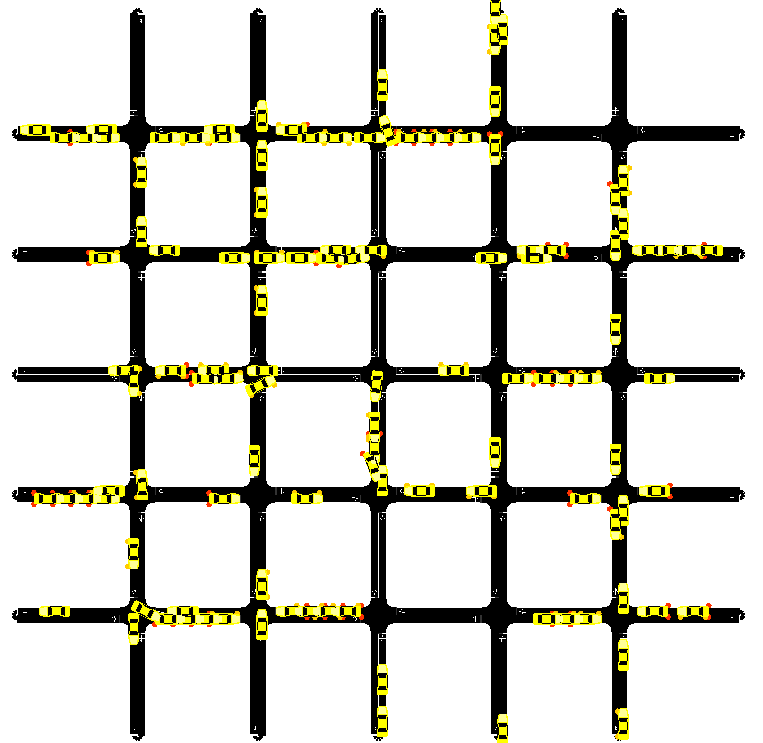
\includegraphics[width=0.4\textwidth]{custom_net}
    \caption{Custom generated $5\times5$ grid network}
    \label{fig:custom_network}
\end{figure}


\begin{table}[h!]
    \centering
    \caption{Tunable parameters of the custom grid network}
    \label{table:grid_params}
    \begin{tabular}{@{} l *4c @{}}
    \toprule
     \multicolumn{1}{c}{Parameter name} & Description \\ 
    \midrule
    Grid Size ($N_G$) & Number of intersections along a single axis of the grid \\ 
    Junction Type & How traffic is regulated at intersections \\ 
    Edge Length ($L_E$) & The distance between two intersections in meters\\
    Number of Lanes ($N_L$) & The number of lanes of each road \\
    Edge Max Speed ($v_{max}$) & The speed limit in the network \\
    \bottomrule
    \end{tabular}
\end{table}

The grids created for our simulation present the parameters shown in Table \ref{table:grid_params}. Intersections are regulated by actuated traffic lights\footnote{Green phases may be prolonged depending on traffic measurements from automatically added induction loops}. Grid size ($N_G$), edge length ($L_E$), and number of lanes ($N_L$) are the parameters that we are interested in varying throughout our simulations.


\subsection{Route Planning}
\label{sec:trip_generation}

In order to simulate traffic flow in the generated network, vehicles' trips that resemble real urban traffic were generated. For this purpose, we used the \verb|randomTrips| tool provided by SUMO, which is able to generate random trips given an input road network, vehicle specification and route properties. This tool automatically ensures that routes and networks are valid. 

\begin{table}[h!]
    \centering
    \caption{Tunable parameters of the vehicle generator}
    \label{table:veh_params}
    \begin{tabular}{@{} l *4c @{}}
        \toprule
        \multicolumn{1}{c}{Parameter name} & Description \\ 
        \midrule
        Vehicle Class  & Vehicle type eg. passenger, emergency, bus \\
        Emissions Class  & Vehicle emissions as per the HBEFA v3.1 standard \\
        Acceleration ($\alpha_V$)  & Maximum vehicle acceleration \\
        Deceleration  & Maximum vehicle deceleration \\
        Max Speed  & Maximum vehicle speed \\
        Speed Factor  & Expected multiplier for lane speed limits \\
        Speed Deviation  & The deviation of the speed factor \\
         \bottomrule
    \end{tabular}
\end{table}

The generator creates vehicles with the properties seen in Table~\ref{table:veh_params}. This allows many different vehicle types to be explored, however, to reduce emulator complexity, only passenger vehicles are generated. Every vehicle has the emission class of a gasoline-driven passenger car (Euro norm 4 HBEFA v3.1-based). Additionally, the maximum deceleration remains constant at $4.5~m/s^2$, the speed factor equals $1$ with a $0.1$ random deviation.

\begin{table}[h!]
    \centering
    \caption{Tunable parameters of the trip generator}
    \label{table:trip_params}
    \begin{tabular}{@{} l *4c @{}}
        \toprule
        \multicolumn{1}{c}{Parameter name} & Description \\ 
        \midrule
        Begin Time ($t_b$)  & Trip departure begin time\\
        End Time ($t_e$)  & Trip departure end time \\
        Period ($\Delta t_V$) & Vehicle departure period \\
        Fringe Factor & Probability multiplier for trips to start on the edge of the network  \\
        \bottomrule
    \end{tabular}
\end{table}

Once the vehicle has been created, trips are generated on the road grid. These trips can be tuned using the parameters seen in Table~\ref{table:trip_params}. Trips depart throughout the simulation time, which has a duration of $300~s$. In order to simulate a grid which is part of a larger network, vehicles are 10 times more likely to start or end their trip on the edge of the network. This is set by the fringe factor. 

\subsection{Tuning congestion}
\label{sec:tuning_congestion}

The shape of the simulated networks varies greatly between different simulations. This is because it is highly dependent on the $N_G$ and $L_E$. Therefore, if we generate the same number of vehicles $N_V$ for every network we will obtain unbalanced traffic congestion throughout the simulations. Small grids are highly congested while large ones have free-flowing traffic. 

In order to keep traffic flow constant between different simulations, we start by defining the total number of roads in the grid $N_{roads}$ and the total number of road meters in the grid $L_{roads}$.

\begin{equation}
    N_{roads} = 2 N_G (N_G - 1) + 4 N_G
\end{equation} 
\begin{equation}
    L_{roads} = N_{roads} L_E
\end{equation}

The maximum number of vehicles $N_{V_{max}}$ that is possible to fit in the simulation will then be:

\begin{equation}
    N_{V_{max}} = \frac{L_{roads}}{\text{Vehicle Length}}
\end{equation}

Finally, to achieve constant traffic density, in each simulation we generate only a percentage of this number by multiplying it by a scaling factor $\beta$. We choose a value of 0.05 for $\beta$ which allows a moderate degree of traffic congestion while avoiding grid-lock.

\begin{equation}
    N_V = \beta  N_{V_{max}}
\end{equation}

Equation~\ref{eqn:num_cars} is used to set the vehicle generation period of the simulation.

\begin{equation}\label{eqn:num_cars}
   \Delta t_V  = \frac{t_e  - t_b}{N_V}
\end{equation}






\section{Experimental Setup}
\label{sec:exp-setup}

Each simulation we ran relied on SUMO, and an interface we wrote allowing us to dynamically vary properties of vehicles, maps and aspects of the environment such as traffic light timing. This allowed us to analyse the effect of various input parameters on various output parameters. For this project, we cared about the following SUMO-generated outputs:

\begin{itemize}
    \setlength\itemsep{0.05em}
    \item average CO$_2$ released per car, per second.
    \item average time lost per second due to driving slower than the ideal speed.
\end{itemize}

We analysed how these outputs were affected by the following inputs:

\begin{itemize}
    \setlength\itemsep{0.05em}
    \item Edge Max Speed, $ 8 \le v_{max} \le 19$ %- legal speed limit in m/s - this \textit{can} be exceeded by vehicles which has a speed-factor greater than 1.
    %\item maxSpeed - the absolute maximum velocity of any vehicle in m/s.
    \item Edge Length, $30 \le L_E \le 70$ %- length of the roads between intersections in meters.
    \item Number of Lanes, $N_L~\epsilon~\{1, 2, 3\}$ %- number of lanes per road.
    \item Grid Size, $N_G~\epsilon~\{3, 4, \dots, 20\}$ %- the number of nodes on each side of the grid (see Section~\ref{sec:map_creation}).
    \item Acceleration, $1.5 \le \alpha_V \le 5$ %- the acceleration ability of vehicles in m/s$^2$.
\end{itemize}

% \harry{This is wrong}
It was important for us to normalize our outputs by a metric that controlled for the size of the grid, because larger grids result in longer travel times, and thus more emissions and lost time. We chose to normalize our outputs by the SUMO-generated ``duration" statistic - the average number of seconds cars were in transit for per simulation. This allowed us to explore more accurately the causal relationship between the above inputs and outputs.

All experiments were conducted using Emukit \cite{emukit2019} - a Python framework for fitting emulators to simulators. Whilst Emukit is agnostic to the underlying statistical model, it has native integration with GPy \cite{gpy2014}, a Gaussian Process framework for Python. Emukit allowed us to conduct Experimental Design, Bayesian Optimisation, and Sensitivity Analysis. % which are used to create and analyse the emulators described in this paper.

% \subsection{Acquisition Functions}
% \label{sec:acquisiton}

% Acquisition functions tell us where to sample our user function. All acquisition functions balance between exploitation and exploration \matteo{carefull, exploitation vs exploration is a concept needed only for bo, where you have to decide if you are happy wiith the minimum you found or explore more as you believe it is a local minimum}\matteo{i would treat the topic of acquiasition functions in the respective sections of ed and bo separately}; some favour sampling regions with high expected variance, whereas others favour regions with known `good' values \cite{siivolaGoodPracticesBayesian2020}. Different acquisition functions are suited to different tasks.

% In the case of experimental design \ref{sec:experimental-design}, where we want to learn as much as possible about the underlying function, we may elect to use uncertainty sampling. Popularised by \cite{lewisHeterogeneousUncertaintySampling1994} \harry{couldn't find the OG paper... todo}, this function selects points which are predicted to produce outputs with high variance. Since Gaussian processes report predictive variance with each evaluation, they are a natural model choice for uncertainty sampling - we can specify an optimizer (usually gradient based) which finds points at which this predictive variance is maximal.

% In the case of Bayesian optimization, where we want to minimize our user function, the `expected improvement' \cite{jonesEfficientGlobalOptimization} acquisition function is more typical. This function samples points which are expected to be lower than the previous best evaluation, whilst still allowing for exploration so as to avoid getting stuck in a local optima. \harry{maybe put a more mathematical definition?}.

% We also considered Thompson sampling and Integrated Variance Reduction. \harry{if we do this}.





\section{Experimental Design}
\label{sec:experimental-design}

% \harry{https://nbviewer.jupyter.org/github/amzn/emukit/blob/master/notebooks/Emukit-tutorial-experimental-design-introduction.ipynb}

% In machine learning, supervised problems are those for which we learn an input-output mapping by fitting some model to a dataset of input-output examples \cite{SupervisedLearning2020}. In many cases, we do not have access to such a dataset, however, we may have the ability to collect input-output pairs on-the-fly. This is the setting where active learning, and indeed experimental design, excel. They use heuristics to guide their choice of input points to evaluate, in the hopes of learning as much as possible about the underlying function, thus enabling us to create an accurate surrogate model of said function. In the context of experimental design, these heuristics are known as acquisitions functions, and in the case where the underlying function is a simulator, we say that the learned surrogate model is an \textit{emulator} if this model also reports how confident it is in its prediction (which is the case for GPs).
%  \harry{is this last sentence true? idk if the defn.is that formal}\matteo{I would drop the last part about reported confidence}

% \subsection{Acquisition Functions}

% Since the purpose of experimental design is to learn as much as possible about the underlying function, we would like an acquisition function that picks points that tell us as much as possible. We experimented with both uncertainty sampling (aka model variance), and integrated variance reduction. Both methods rely on being able to evaluate the predictive variance of our model with respect to any particular input; since GPs report this with each evaluation, they are a natural model choice for both uncertainty sampling and integrated variance reduction. Also, both methods rely on gradient-based optimizers to find the next point in the domain for which the respective measure is either maximised (in the case of uncertainty sampling) or minimized (in the case of integrated variance reduction) \cite{EmukitExperimentalDesign2020}.


% Uncertainty sampling \cite{lewisHeterogeneousUncertaintySampling1994}, selects points for which the current emulator prediction has high variance, with the rationale being that points with high variance are `interesting' and have more to be learned from than points we're already confident about. More formally, we wish to find points $\mathbf{x}$ at which the predictive variance $\sigma^{2}(\mathbf{x})$ of our model is maximal. In theory, high-variance regions of your learned function will be sampled frequently and therefore have their variance reduced. This should drive us to explore different points in the input domain which have greater predictive variance.
We performed experimental design with both uncertainty sampling (aka model variance) and integrated variance reduction. We found that uncertainty sampling was prone to a sort of `reward hacking' \cite{hadfield-menellInverseRewardDesign2020}. Our optimization continually collapsed to finding a configuration of 4/5 input parameters that produced extremely high variance when varying the remaining 1/5 parameter (`edgeLength', the length of roads between intersections, was this parameter). This meant that it failed to learn an accurate model of the underlying function, instead learning only about that one parameter. We originally attributed these highly variable outputs to a bug in our underlying simulation, which the experimental design process had learned to exploit. However, even after fixing this, uncertainty sampling still favoured extreme points in the input domain. This makes sense since the point of uncertainty sampling is to find points with high variance, however, this was not ideal for us; we wanted confident predictions across the full input domain, not just at the extremes.

Integrated variance reduction (IVR) \cite{sacksDesignAnalysisComputer1989} proved to be more effective for our purposes. We found that IVR was less prone to `reward hacking', and explored the parameter space more completely - this is reflected in our results.

% This acquisition function lets us finds points in the input domain which reduce the total variance of the model, where the total variance is computed using Monte-Carlo integration over some fixed number of randomly sampled points $\mathbb{X}$, given a prospective input point $\mathbf{x}$. The Monte-Carlo approximation takes following form \cite{EmukitExperimentalDesign2020}. \harry{This is copied https://mlatcl.github.io/mlphysical/lectures/04-02-emukit-and-experimental-design.html - is this acceptable w/ citation?}\nicholas{Probably not. Though there should be citations at the bottom of the page}


% \begin{equation}
% \begin{aligned}
% a_{I V R} &=
% & \approx \frac{1}{\# \text { samples }} \sum_{i}^{\text {# } \operatorname{samples}}\left[\sigma^{2}\left(\mathbf{x}_{i}\right)-\sigma^{2}\left(\mathbf{x}_{i} ; \mathbf{x}\right)\right]
% \end{aligned}
% \end{equation}

% Reiterating, prospective points $\mathbf{x}$ are computed by performing gradient descent to minimise $a_{I V R}$. We found that IVR was less prone to `reward hacking', and explored the parameter space more completely. % - this is reflected in our results.

\subsection{Experimental Design Results}


% \harry{permutations: Model\_variance timeloss, model\_variance co2, thompson sampling timeloss, thompson sampling co2 }

To assess the efficacy of our learned emulators, and experimental design in general, we performed t-tests in which we compared emulators learned using principled acquisition functions (uncertainty sampling and integrated variance reduction) to emulators learned using randomly sampled points. To do this, we first collected two sets of randomly sampled points using Emukit's `RandomDesign' utility; an initialization set of 20 points to initialize each GP with, and a test set of 100 points to evaluate the mean squared error of our models against. Then, we trained three emulators; one using uncertainty sampling (model\_variance) as our acquisition function, one using integrated variance reduction, and one using randomly sampled points. Every 50 iterations we evaluated each model on our test set - these results are plotted in Figure~\ref{fig:exp-design-loss}, please note that y-axes are on different scales. 

After all models had `seen' 500 points, we computed for each a final root mean squared error. Our results are summarised thus:

\begin{itemize}
    \item Integrated Variance Reduction was 13.98\% better than training on randomly sampled points when modelling CO2 per second.
    \item Integrated Variance Reduction was 7.63\% better than training on randomly sampled points when modelling time loss per second.
    \item Uncertainty Sampling was -8.25\% worse than training on randomly sampled points when modelling CO2 per second.
    \item Uncertainty Sampling was 2.58\% better than training on randomly sampled points when modelling time loss per second.
\end{itemize}

\begin{figure}[b!]
    \centering
    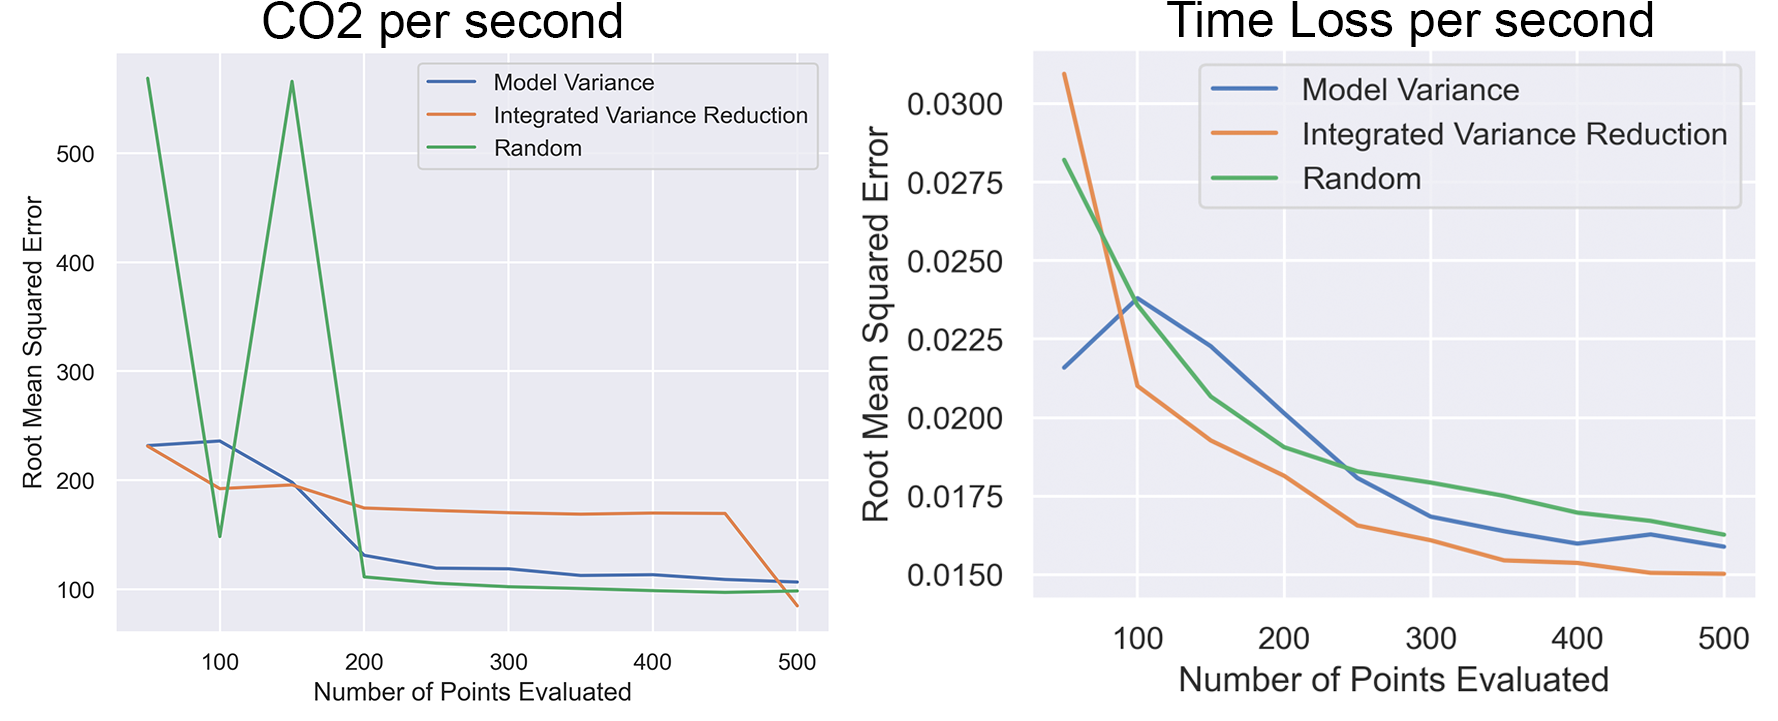
\includegraphics[width=0.9\textwidth]{images/exp_design_graph.png}
    \caption{Experimental Design results - root mean square error for models trained on intervals of 50 points acquired through uncertainty sampling (model variance), integrated variance reduction, and random sampling.}
    \label{fig:exp-design-loss}
\end{figure}

These results show that acquisition through integrated variance analysis is beneficial for our particular problem, however, acquisition through uncertainty sampling is less effective. The advantage of both acquisition functions diminishes relative to random sampling as more and more points are collected, implying that these techniques excel in settings where we have few input points. We ran experimental design 5 times for both CO2 and TimeLoss, then chose the lowest RMSE emulators to pass onto Bayesian Optimization. 
% All 5 runs produced similar RMSE models.


\section{Bayesian Optimization}
\label{sec:bay_opt}



How can we reduce traffic congestion? Can we structure our road networks so that navigation is both fast and the impact on the environment is reduced? In this section, we investigate these questions trying to provide answers based on our traffic emulator.

We are interested in finding the optimal parameters' configuration in order to minimise our outputs. However, the function we aim to optimise is explicitly unknown and querying it for a single data point takes a few seconds. For this reason, we use Bayesian Optimisation (BO), already introduced in section \ref{sec:bo_background}. In this work, we choose Expected Improvement as our acquisition function. Optimisation is ran on the models acquired from experimental design (\ref{sec:experimental-design}).

The resulting optimal points can be seen in Table \ref{table:optimal_points}. We observe that for both models the lowest output is found with minimum speed and maximum road length. Intuitively, navigating networks with shorter roads implies spending more time traversing intersections, which are a major source of delay and pollution in cities. The low speed limit benefits emissions as it implies that less trip time will be spent accelerating. We also see that more lanes benefit time loss while fewer lanes are better to optimise emissions. This is intuitive as lane changes are known to increase pollution \cite{rakha2000requirements}. Finally, the optimal acceleration to optimise emissions may be an unexpected result, but we know that a vehicle's emission efficiency curve is never zero. Thus, a lengthy, low acceleration trip may emit more CO$_2$ than a short, erratic one.

\begin{table}[h!]
    \centering
    \caption{Optimal parameters' configurations found with Bayesian Optimisation}
    \label{table:optimal_points}
    \begin{tabular}{@{} l *5c l c @{} }
    \toprule
    \multicolumn{1}{c}{Emulator}  & $N_G$ &  $v_{max}$ & $L_E$ & $N_L$ & $\alpha_V$ & Output \\ 
    \midrule
        Time loss & 10 & 8 & 70 & 2 & 1.86 & 12.37\\
        Emissions & 20 & 8 & 61.36 & 1 & 2.96 & 1721.50\\
    \midrule
        Average & 15 & 8 & 65.68 & 1 & 2.28 & \\
    \bottomrule
    \end{tabular}
\end{table}

We investigate more deeply the grid size. We observe that the two models pick very different grid size values, this suggests that there could be a trade-off related to the grid size and that optimising this size for both objectives is pareto-optimal. For this purpose, we analyse the simulator and the emulators in the average optimal point shown in Table \ref{table:optimal_points}.
In Figure~\ref{fig:trade_off} we observe that indeed this trade-off exists in the simulator and our emulators are able to capture it. This gives insights on the fact that when planning urban areas the size of the network is a crucial factor. Choices that benefit travel time may pose a danger for the environment.

\begin{figure}[b!]
\centering
\begin{subfigure}{0.5\textwidth}
  \centering
  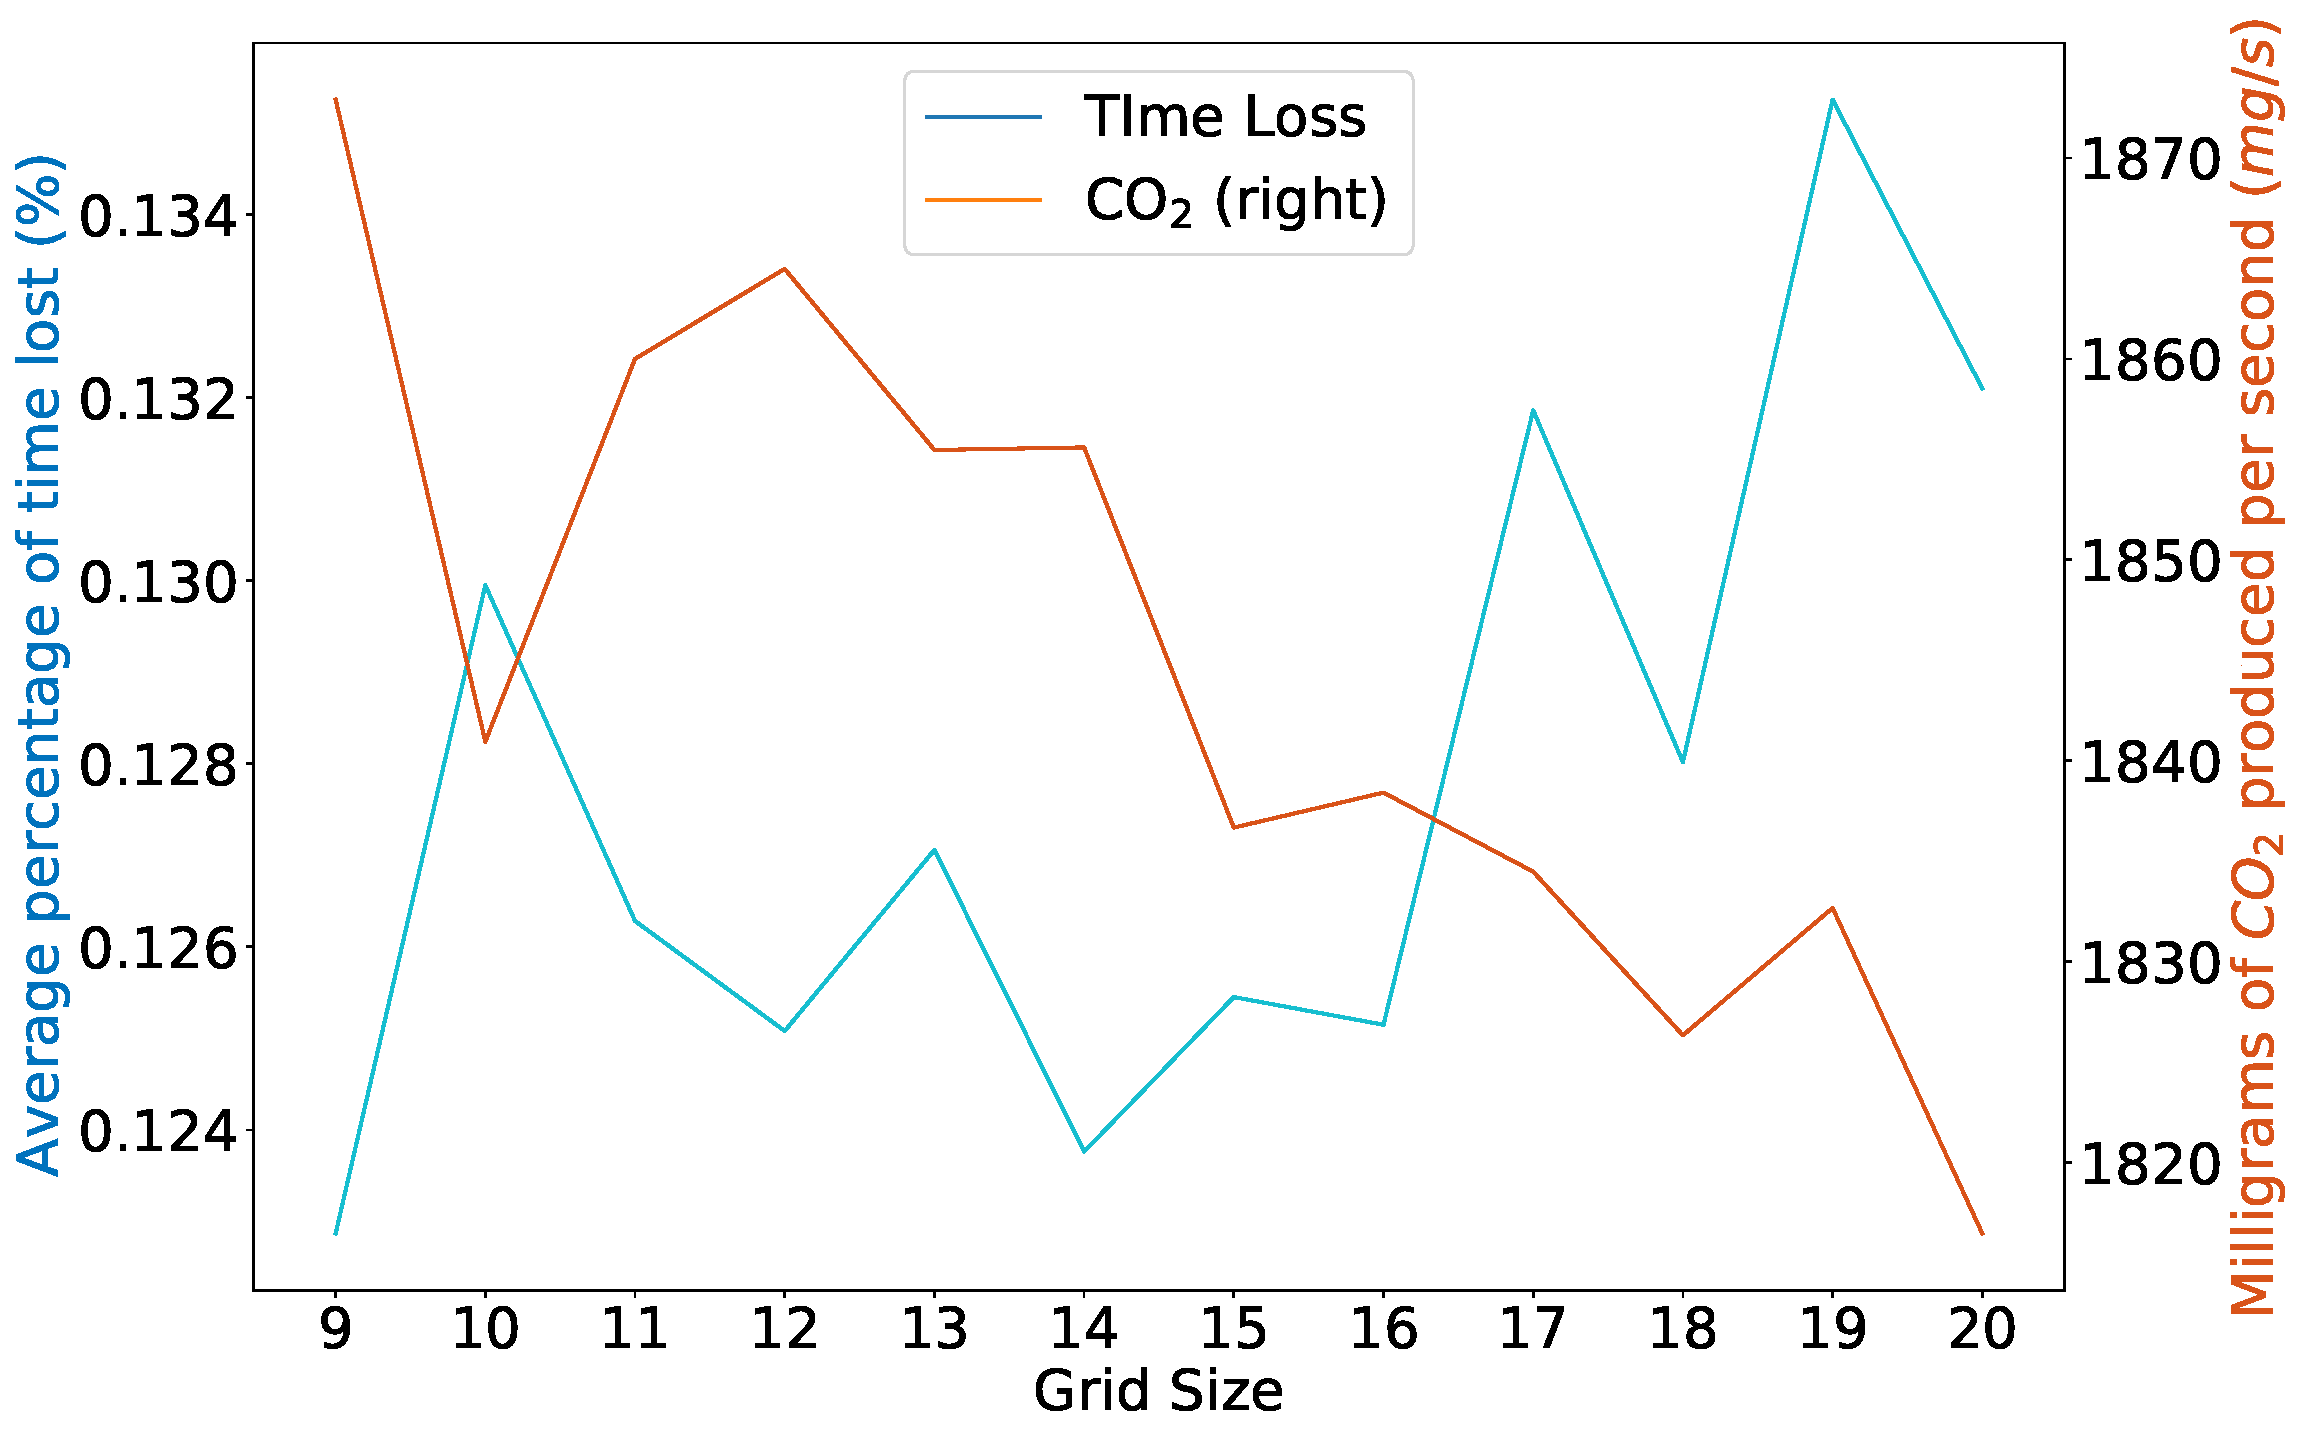
\includegraphics[width=\textwidth]{trade-off_simulator_gridSize}
  \caption{Simulator}
\end{subfigure}%
\begin{subfigure}{0.5\textwidth}
  \centering
  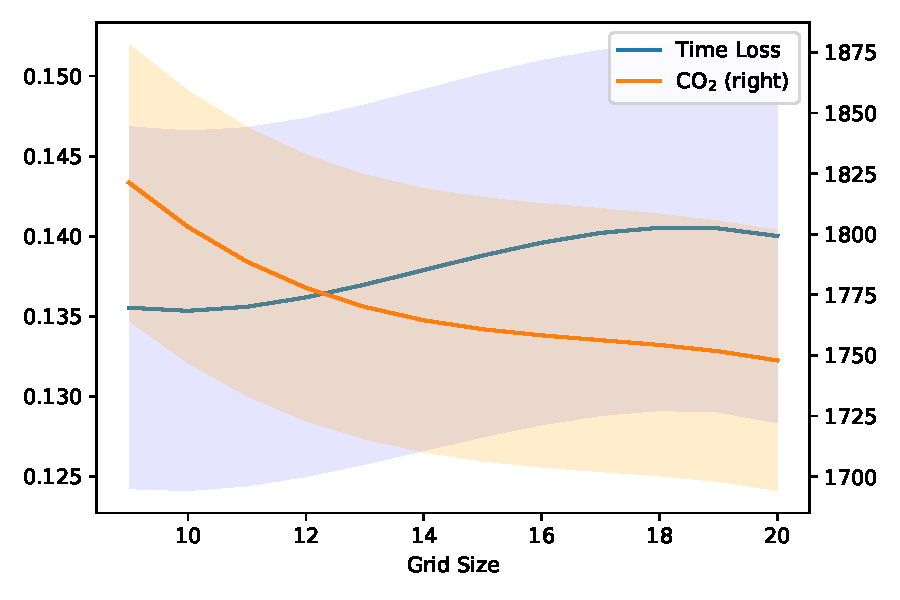
\includegraphics[width=\textwidth]{small_grid_size}
  \caption{Emulator}
\end{subfigure}
\caption{Trade-off between CO$_2$ and time loss when varying the grid size in the average optimal point}
\label{fig:trade_off}
\end{figure}

Finally, as we run Bayesian optimisation on the experimentally designed emulators, we aim to compare the difference between the emulators before and after the optimisation phase. In Figure~\ref{fig:grid_size_comp} we see that for grid size the predictive variance decreases significantly and also the prediction mean is subject to modification. For further comparisons please refer to Appendix~\ref{appendix:comparison}.

\begin{figure}[t!]
\centering
\begin{subfigure}{0.5\textwidth}
  \centering
  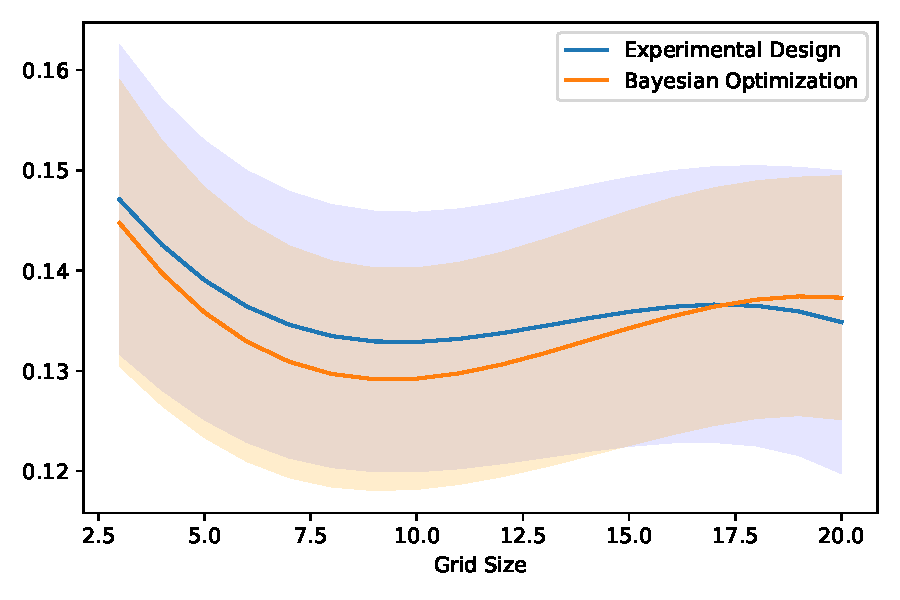
\includegraphics[width=\textwidth]{images/ofat_compare/time/grid_size.pdf}
  \caption{Time loss}
\end{subfigure}%
\begin{subfigure}{0.5\textwidth}
  \centering
  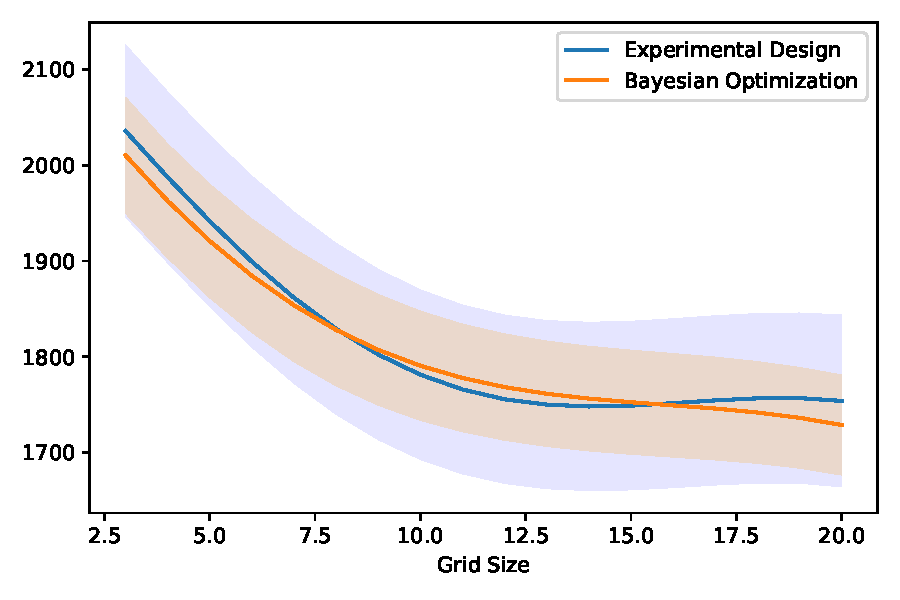
\includegraphics[width=\textwidth]{images/ofat_compare/co2/grid_size.pdf}
  \caption{CO$_2$}
\end{subfigure}
\caption{Experimental design and Bayesian Optimisation model comparison for grid size in the average optimal point}
\label{fig:grid_size_comp}
\end{figure}


\section{Sensitivity Analysis}
\label{sec:sensitivity_analysis}

In order to determine the significant inputs, sensitivity analysis is completed on the optimised emulators. Analyses are completed independently for time-loss and CO$_2$ emissions. This allows the important factors for each output to be discovered. OFAT and Global Sensitivity analysis are completed on each emulator.

\begin{figure}[b!]
    \centering
    \begin{subfigure}[b]{0.49\textwidth}
        \centering
        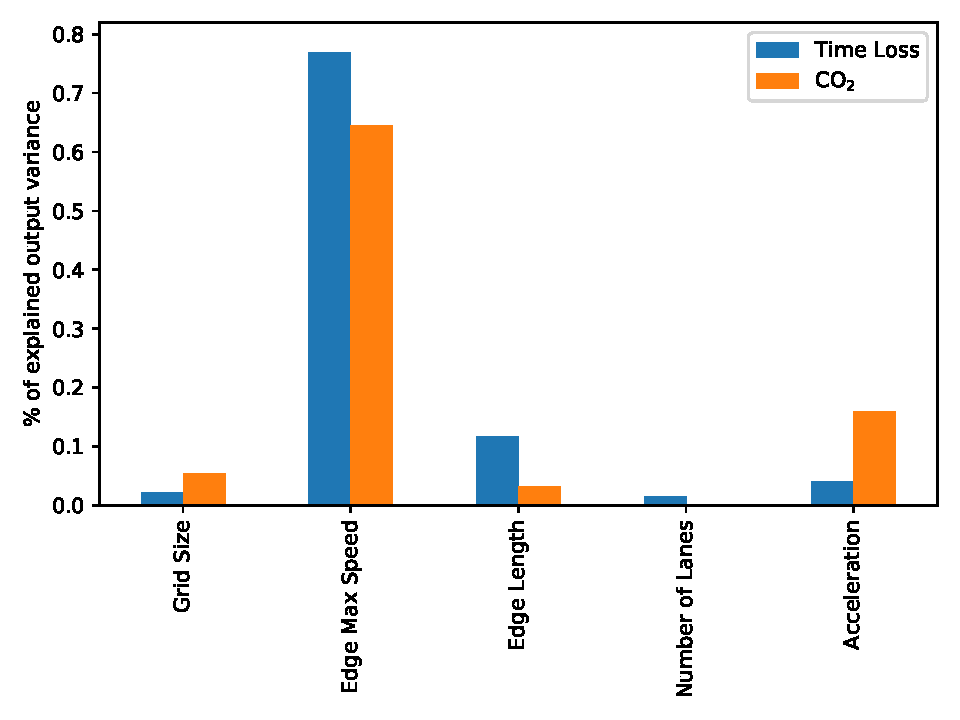
\includegraphics[width=\textwidth]{images/main_effects.pdf}
        \caption{Main Effects}
        \label{fig:main_effects}
    \end{subfigure}
    \hfill
    \begin{subfigure}[b]{0.49\textwidth}
        \centering
        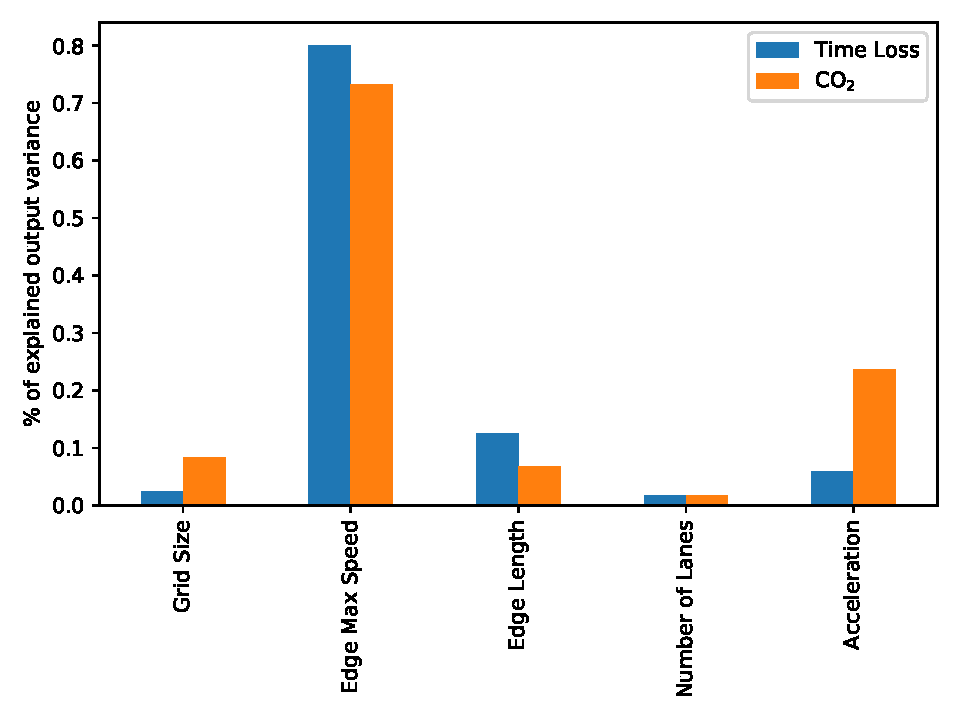
\includegraphics[width=\textwidth]{images/total_effects.pdf}
        \caption{Total Effects}
        \label{fig:total_effects}
    \end{subfigure}
    \caption{Comparison of Sobol indices obtained from the time loss and $CO_2$ emulators}
    \label{fig:sobol}
\end{figure}

\begin{figure}[t!]
    \centering
    \begin{subfigure}[b]{0.49\textwidth}
        \centering
        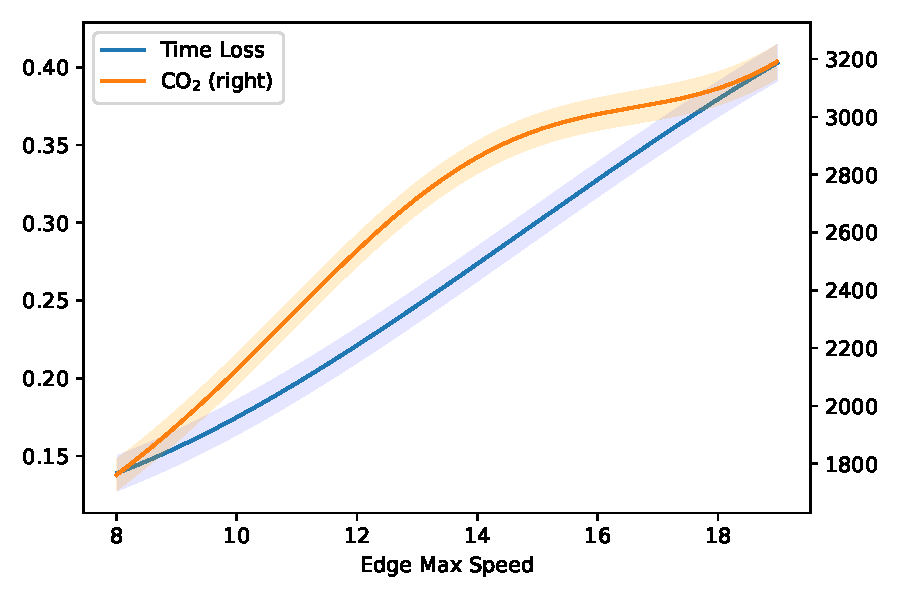
\includegraphics[width=\textwidth]{images/edge_max_speed.pdf}
        \caption{Edge Max Speed $v_{max}$}
        \label{fig:edge-max-speed}
    \end{subfigure}
    \hfill
    \begin{subfigure}[b]{0.49\textwidth}
        \centering
        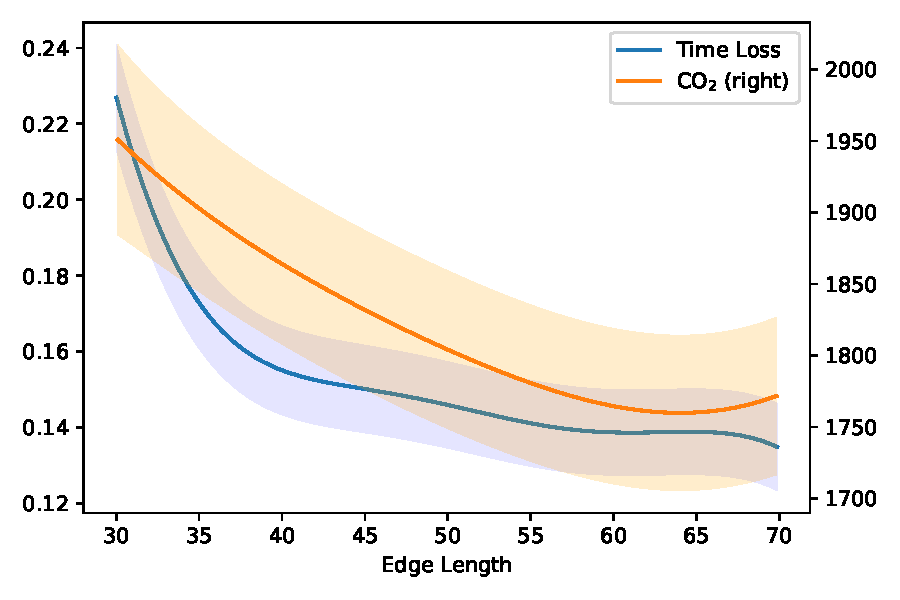
\includegraphics[width=\textwidth]{images/edge_length.pdf}
        \caption{Edge Length $L_E$}
        \label{fig:edge-length}
    \end{subfigure}
    \hfill
    \begin{subfigure}[b]{0.49\textwidth}
        \centering
        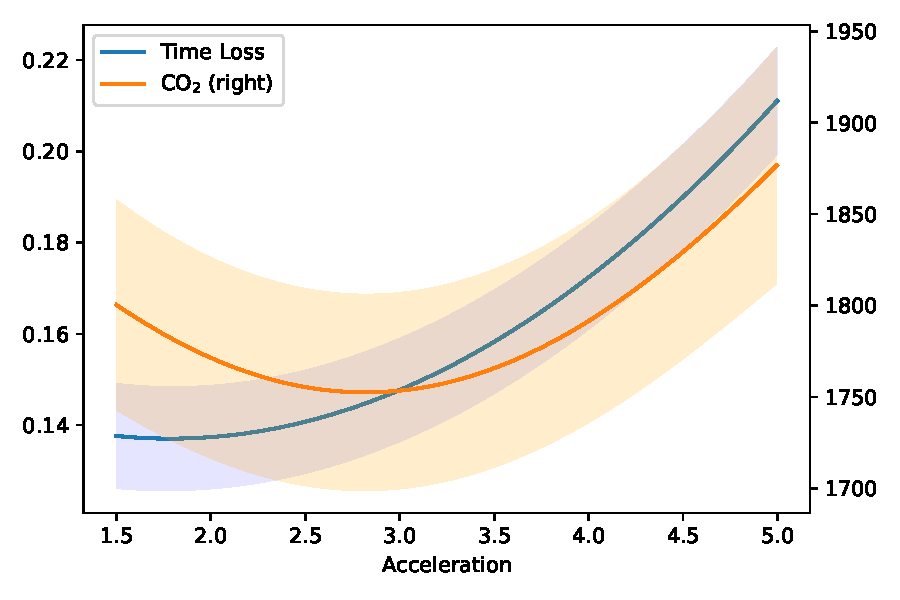
\includegraphics[width=\textwidth]{images/acceleration.pdf}
        \caption{Maximum Acceleration $\alpha_V$}
        \label{fig:acceleration}
    \end{subfigure}
    \caption{OFAT comparison of the emulators at the average operating point. Filled areas show one standard deviation of model variance.}
    \label{fig:ofat}
\end{figure}

The first-order indices and total effects of each input variable is calculated for both emulators. This is completed using a model-based Monte-Carlo approach with $500000$ iterations. The OFAT analysis is conducted by randomly sampling 500 data-points for each input from the parameter space. All other parameters remain constant and are set to the average optimal operating point seen in Table~\ref{table:optimal_points}.

Figure~\ref{fig:sobol} shows that edge max speed is the most significant input parameter to the system, as it contributes to more than half of the output variance. The other input parameters have very little impact on the system. Two exceptions are edge length in the time loss emulator, and acceleration in the CO$_2$ emulator. Figure~\ref{fig:ofat} shows the OFAT analysis of these input parameters, in which it can be seen that time loss is proportional to emissions.

These results allow us to make interesting observations. High $v_{max}$ in an urban environment results in both high time losses and emissions. Time loss is increased because vehicles reach road junctions faster, and thus have to wait longer to proceed on their journey, which emissions are increased due to extended acceleration periods. Rapid acceleration and deceleration is considered a poor and dangerous driving practice. Figure~\ref{fig:acceleration} shows that this behaviour results in more time loss than if one were driving moderately. 


\section{Future Work}

Due to resource constraints, the emulators were developed using a limited number of initialisation and iteration datapoints. By increasing the number of datapoints used, the fidelity of the emulators can be increased. 

Many cities are extremely large and dense, which can be simulated by larger grid sizes. Further research in this field can take these larger grids into account. Larger cities also incorporate multi-modal traffic. Future investigations in this area can include other vehicles such as public transport, pedestrians, and emergency vehicles. 

To further test the advantages of microscopic traffic emulation, comparisons between mesoscopic traffic models and microscopic emulators could be done.

\section{Conclusion}
\label{sec:conclusion}

Two traffic emulators were designed for use in urban traffic management and road planning. These emulators are designed to model the time loss due to driving below the ideal speed, and CO$_2$ emissions. The emulators use gaussian processes as a surrogate model of a microscopic traffic simulator SUMO, developed using experimental design techniques. It was found that the Integrated Variance Reduction produced the models with the smallest RMSE using 20 randomly initialised points, followed by the experimental design loop with 500 iterations. 

In order to find the minimum-output operating point for each emulator, Bayesian Optimisation with Expected Improvement point acquisition was used. The minimum operating points were very similar. The operating points are investigated using sensitivity analysis. It was found that the most significant parameter is the edge maximum speed, followed by edge length and maximum acceleration for time loss and CO$_2$ emissions respectively. 

The analysis shows that low vehicle speeds in combination with long edges give ideal time loss and emission performance. Additionally, by increasing the number of road lanes, there is less time loss in the network. An important trade-off between time loss and emissions is also discovered when varying the network size. This pareto-optimality can lead to useful insights for urban planners.

\newpage
\bibliographystyle{unsrt}
\bibliography{lib.bib}

\newpage
\begin{appendices}
\section{Comparing OFAT between experimental design and Bayesian Optimisation}
\label{appendix:comparison}


In this appendix we report the comparison between the emulators before and after Bayesian Optimisation. On the left side time loss is shown while on the right sides CO$_2$ emission is shown.


\begin{figure}[h!]
\centering
\begin{subfigure}{0.5\textwidth}
  \centering
  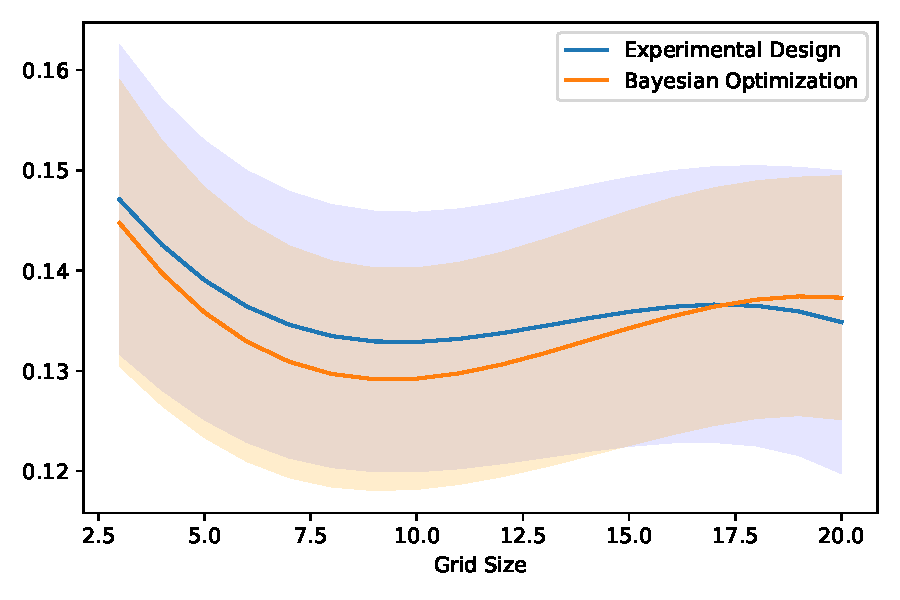
\includegraphics[width=\textwidth]{images/ofat_compare/time/grid_size.pdf}
\end{subfigure}%
\begin{subfigure}{0.5\textwidth}
  \centering
  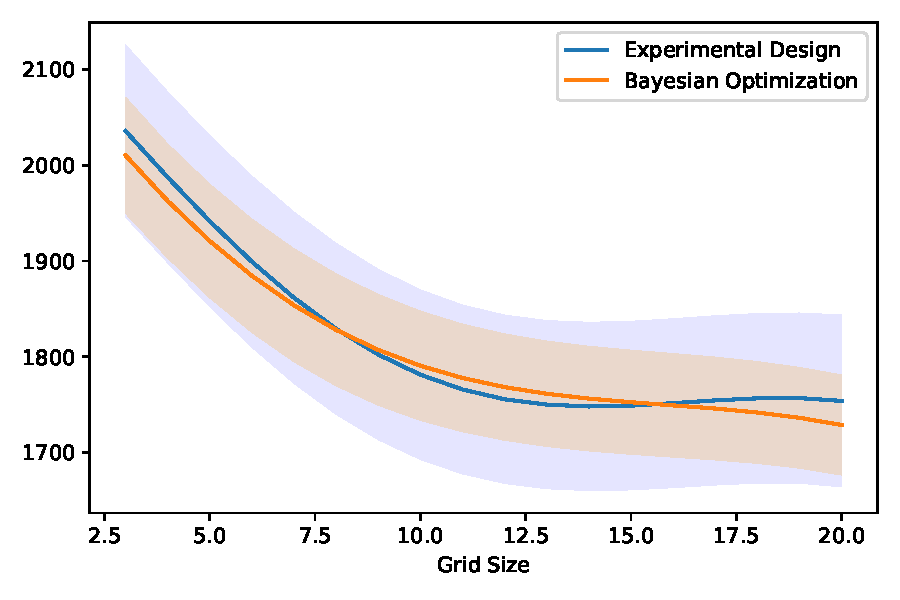
\includegraphics[width=\textwidth]{images/ofat_compare/co2/grid_size.pdf}
\end{subfigure}
\caption{Grid size}
\end{figure}

\begin{figure}[h!]
\centering
\begin{subfigure}{0.5\textwidth}
  \centering
  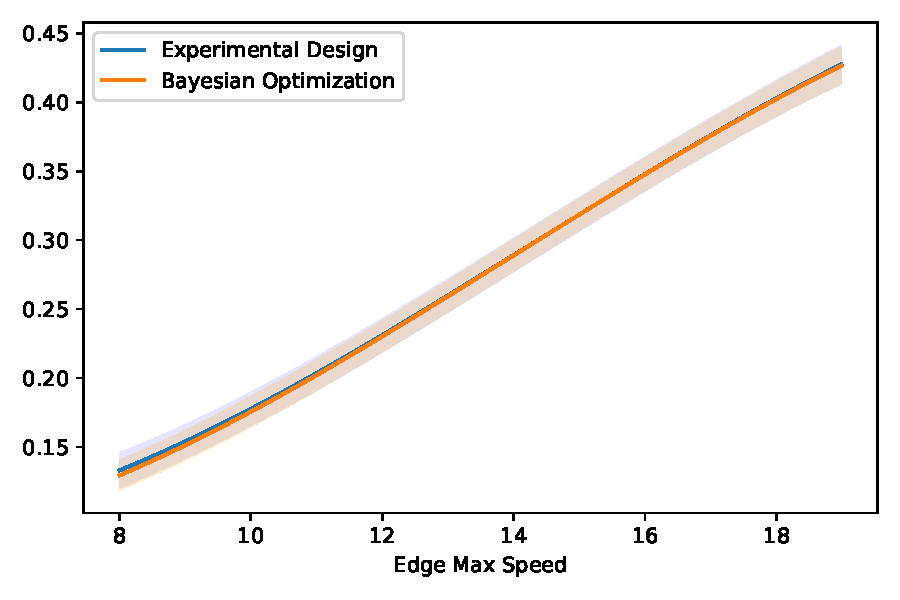
\includegraphics[width=\textwidth]{images/ofat_compare/time/edge_max_speed.pdf}
\end{subfigure}%
\begin{subfigure}{0.5\textwidth}
  \centering
  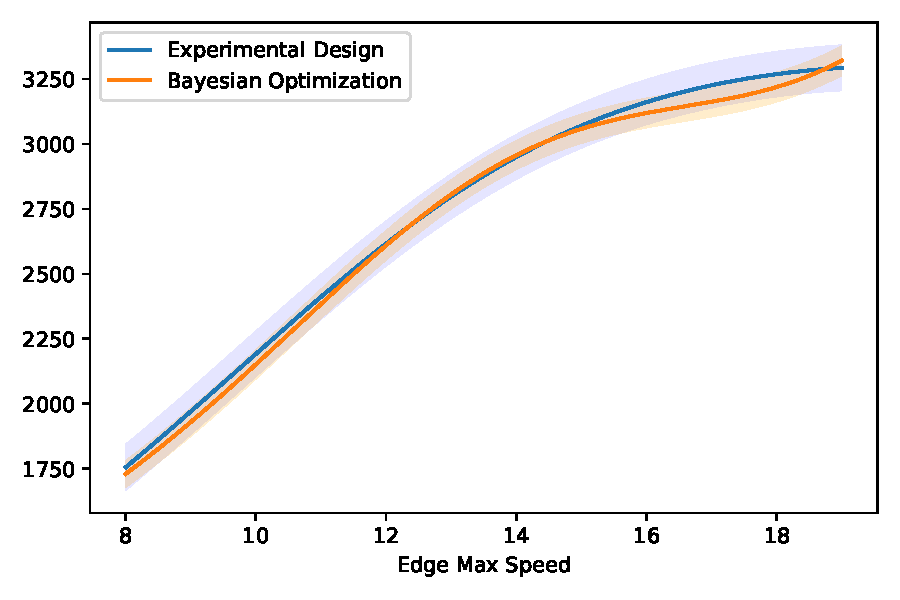
\includegraphics[width=\textwidth]{images/ofat_compare/co2/edge_max_speed.pdf}
\end{subfigure}
\caption{Road max speed}
\end{figure}


\begin{figure}[h!]
\centering
\begin{subfigure}{0.5\textwidth}
  \centering
  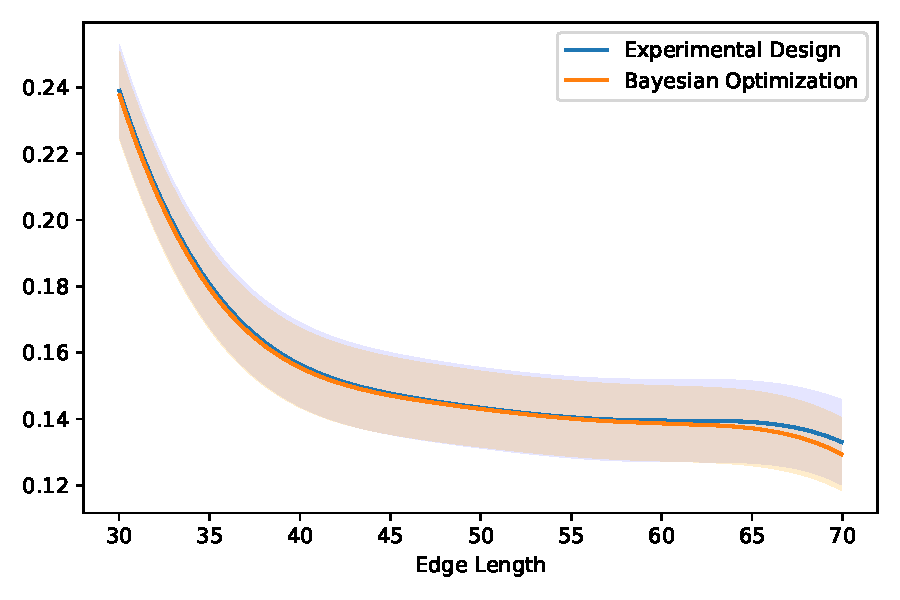
\includegraphics[width=\textwidth]{images/ofat_compare/time/edge_length.pdf}
\end{subfigure}%
\begin{subfigure}{0.5\textwidth}
  \centering
  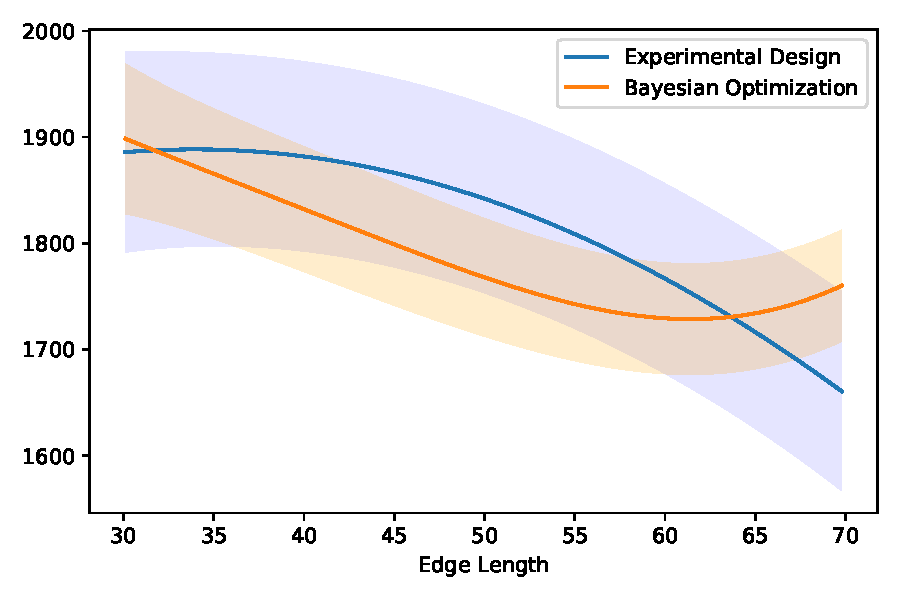
\includegraphics[width=\textwidth]{images/ofat_compare/co2/edge_length.pdf}
\end{subfigure}
\caption{Road length}
\end{figure}

\begin{figure}[h!]
\centering
\begin{subfigure}{0.5\textwidth}
  \centering
  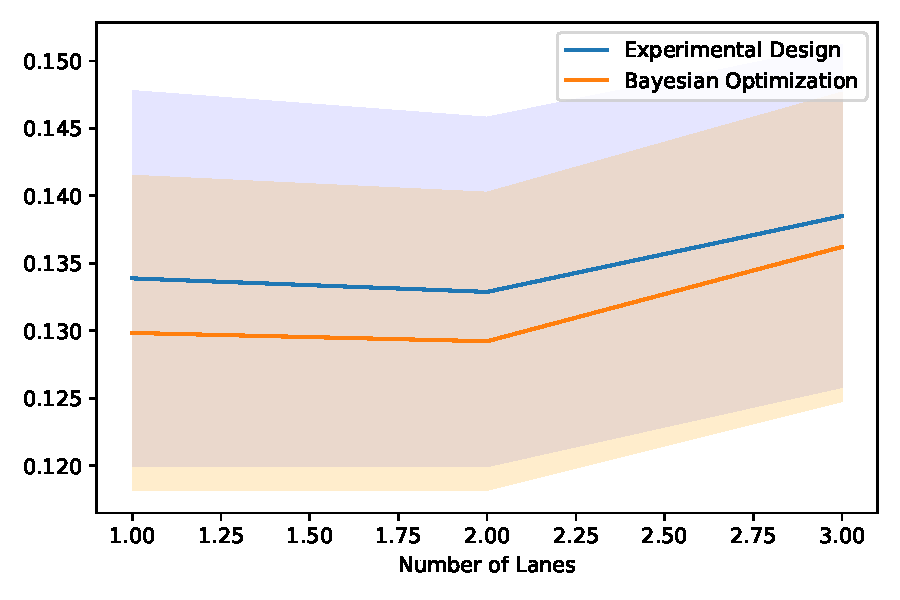
\includegraphics[width=\textwidth]{images/ofat_compare/time/number_of_lanes.pdf}
\end{subfigure}%
\begin{subfigure}{0.5\textwidth}
  \centering
  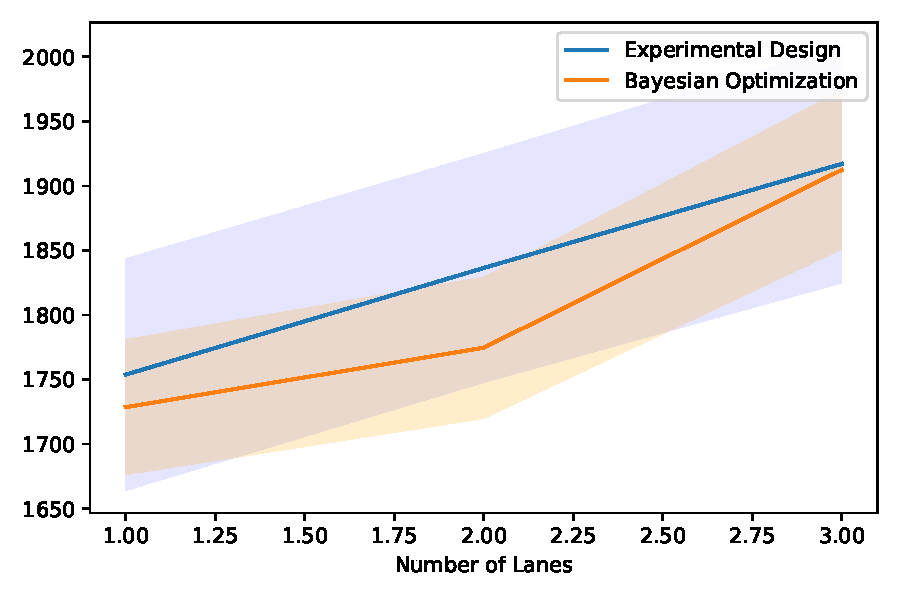
\includegraphics[width=\textwidth]{images/ofat_compare/co2/number_of_lanes.pdf}
\end{subfigure}
\caption{Number of lanes}
\end{figure}

\begin{figure}[h!]
\centering
\begin{subfigure}{0.5\textwidth}
  \centering
  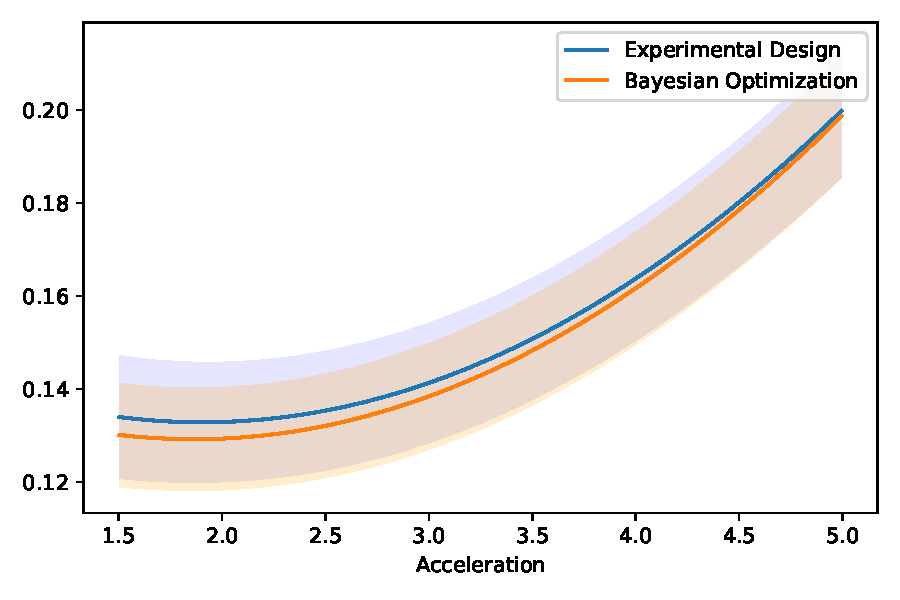
\includegraphics[width=\textwidth]{images/ofat_compare/time/acceleration.pdf}
\end{subfigure}%
\begin{subfigure}{0.5\textwidth}
  \centering
  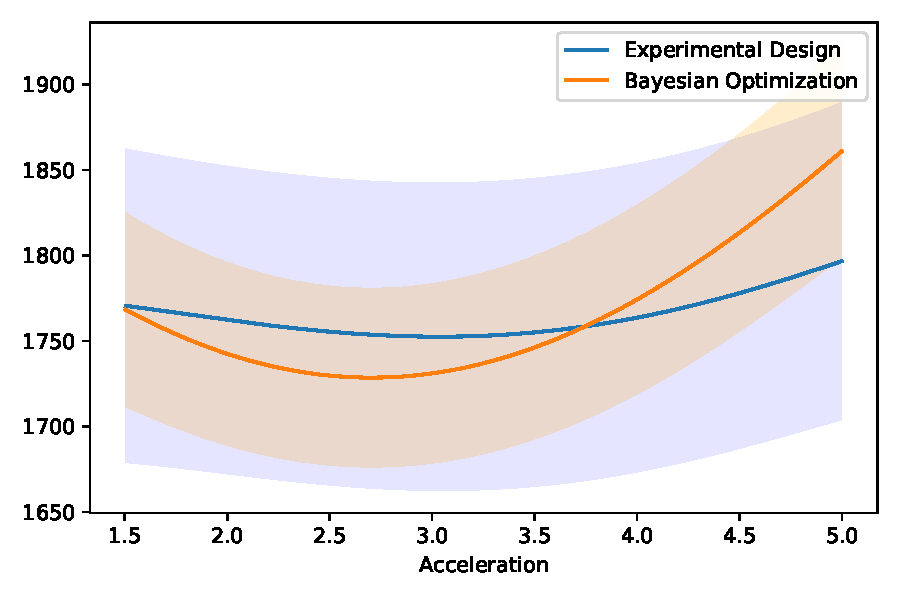
\includegraphics[width=\textwidth]{images/ofat_compare/co2/acceleration.pdf}
\end{subfigure}
\caption{Acceleration}
\end{figure}

\end{appendices}
\end{document}